\documentclass[12pt,a4paper,oneside]{article} % part, *section, *paragraph
%\documentclass[12pt,a4paper,oneside]{report} % part, *chapter, *section, *paragraph
%\documentclass[12pt,a4paper,oneside]{book} % part, *chapter, *section, *paragraph

\usepackage[english]{babel}
\usepackage[latin2]{inputenc}
\usepackage{setspace}
\usepackage{float}
\usepackage[T1]{fontenc} %\showhyphens{integetnem} \showhyphens{meggy�ltetv�ny}
%\usepackage{ucs}\usepackage[utf8x]{inputenc}
%\usepackage{fullpage} %\usepackage[margin=2cm]{geometry}
%\usepackage{amsmath,amssymb}
\usepackage{url} %VAGY %\usepackage[unicode]{hyperref}
\usepackage{listings}
%\usepackage{color} 
\usepackage{graphicx}
\usepackage{times}
\usepackage{fullpage}
%\usepackage{showkeys} % \label{} ki�r�sa \ref{}hez
 
\let\stdsection\section
\renewcommand\section{\clearpage\stdsection}
\begin{document}
\onehalfspacing
\begin{center}
\vspace{2em}
%\large{\bf{}BUDAPESTI M\H{U}SZAKI \'ES GAZDAS\'AGTUDOM\'ANYI EGYETEM}
\vspace{.5em}


\includegraphics[width=60mm]{10000000000004C00000014A5D3CE278.eps}

Budapest University of Technology and Economics

Department of Measurement and Information Systems
%\vspace{.5em}

%\large{\bf{}VILLAMOSM\'ERN\"OKI \'ES INFORMATIKAI KAR\\
%M\'ERN\"OK INFORMATIKUS SZAK}

\vspace{2em}

%\Large{Informatikai Technol\'ogi\'ak szakir\'any\\
%Rendszerfejleszt\'es \'agazat}

%\vspace{1.5em}

%\Large{\bf{}\"On\'all\'o labor (BMEVIIIA337)}

%\vspace{1.5em}

\LARGE{\bf{}RTF tokenizer for LibreOffice writerfilter (rewrite of the RTF import)}

\vspace{2em}

\begin{tabular}{ l c}
  %hopefully i can avoid the photo this time
  %\parbox{30mm}{\includegraphics[width=20mm]{20090926.eps}} &
  \parbox{120mm}{
\begin{center}
\normalsize{Vajna Mikl�s (AYU9RZ),

4th semester, (MSc) computer engineering student

Consultants: C�dric Bosdonnat, M�t� Andr�s, Novell

Internal consultant: Horv�th �kos, MIT

Specialization in Dependable System Design

Internship Report

2011/12. 1st semester}
\end{center}
} \\
\end{tabular}


\end{center}
\thispagestyle{empty}
\newpage

\tableofcontents
\newpage

\section{Introduction}

LibreOffice is a power-packed free, libre and open source personal
productivity suite for Windows, Macintosh and GNU/Linux, that gives you six
feature-rich applications for all your document production and data processing
needs: Writer, Calc, Impress, Draw, Math and Base\cite{libreoffice}.

During my internship I worked on Writer. Writer has support for lossless import
and export from/to the ODF file format (.odt). Additionally, several other
filters are supported which are marked as ``alien'': such filters may lose some
information upon loading/saving. Such an alien RTF\cite{rtf} filter was already
implemented in LibreOffice 3.4, and my task was to improve it.

The source code of LibreOffice is divided to several (at the time of writing:
225) modules, two of them is \emph{writerfilter}, which contains the import
filter for the DOCX file format and \emph{sw}, the module of Writer
application.

At the begining, the writerfilter module already contained code to map
Microsoft Office's concepts to LibreOffice's ones (for example Microsoft Office
uses section breaks for different page settings, LibreOffice uses page styles
for that purpose, etc.), and an internal RTF import filter within the sw module
did something similar, but without less features.

In this paper I represent my work on re-writing the RTF filter in the
writerfilter module, getting rid of code duplication and adding support for
mappings which were missing in the old RTF filter.

The rest of this paper is structured as follows. First, I introduce necessary
background knowledge, which was present before the current paper, but is needed
to understand the rest of this work (Section 2). Section 3 describes the design
of the solution, as well as relation with the underlying techniques. Next, I
detail the implementation I created (Section 4). After that, I evaluate the
created module (Section 5). Finally I give a summary, including future
development directions (Section 6).

\section{Background}

A filter in LibreOffice is a class, that implements given interfaces, and
performs the import or the export (or both) of a file format to one of the six
applications.

Registrations of such classes are usually handled via UNO (Universal Network
Objects), the interface based component model of LibreOffice.\footnote{Old
filters are not using UNO and are bundled together with applications (e.g.
Writer).} Each filter has a configuration file, which lists the file format
detector service and the filter service.

I did not have to pay attention to the RTF file format detector service, as it
was already working and I had no plans to improve it. The filter was an UNO
one, but the import part of it was just a stub, that called the old RTF
importer, that was a builtin one.

Implementing a filter via UNO has multiple advantages:

\begin{itemize}
\item The applications are written in C++, but the implementation of UNO services can be anything supported by UNO (e.g. Java or Python).
\item The filter can be built once the UNO interfaces implemented by the
application are available, even if the source code of the application it not
available\footnote{This may be strange as a goal for a free software project,
but given that LibreOffice is huge and building it is non-trivial, it's
useful.}.
\end{itemize}

The already cited RTF specification defines the major tasks of an RTF reader:

\begin{itemize}
\item Separate text from RTF controls.
\item Parse an RTF control.
\item Dispatch an RTF control.
\end{itemize}

Separating text from RTF controls is relatively simple: all RTF controls begin
with a backslash and can contain a defined set of characters only.

Parsing an RTF control is also relatively simple: RTF defines different type of
control words and each of them a simple rule of what type of parameters can
they take (if any).

Dispatching an RTF control, on the other hand, is relatively complicated: once
needs having a really good knowledge of the API of the target application,
since most of the RTF control words will result in an API call, passing the
parameters of the control word to the document model.

Next to control words, RTF has the concept of groups. They start with a
\textbraceleft and end with a \textbraceright -- and they should be threated
like a stack: the scope of control words starts where they appear and ends at
the end of the current group.

RTF defines the following control word types:

\begin{itemize}
\item flags: they take no parameter, for example \textbackslash{}sbknone
\item destinations: these appear at the start of a group and if they are
	ignored, the whole group should be ignored, for example \textbackslash{}fonttbl
\item symbols: they don't take parameters, either -- special symbols like \textbackslash{}tab have this type
\item toggles: they switch a property on or off, for example bold characters are marked using \textbackslash{}b
\item value: they always take a parameter, for example font size (\textbackslash{}fs)
\end{itemize}

Now that we are aware of basic concepts of RTF, the next section overviews the
API requirements of Writer and explains the design of the filter that can parse
and RTF document.

\section{Design}

The design of the RTF filter is determined by the requirements from the RTF
specification and the interfaces provided by the domain mapper.

The control flow has the following architecture:

\begin{figure}[H]
\centering
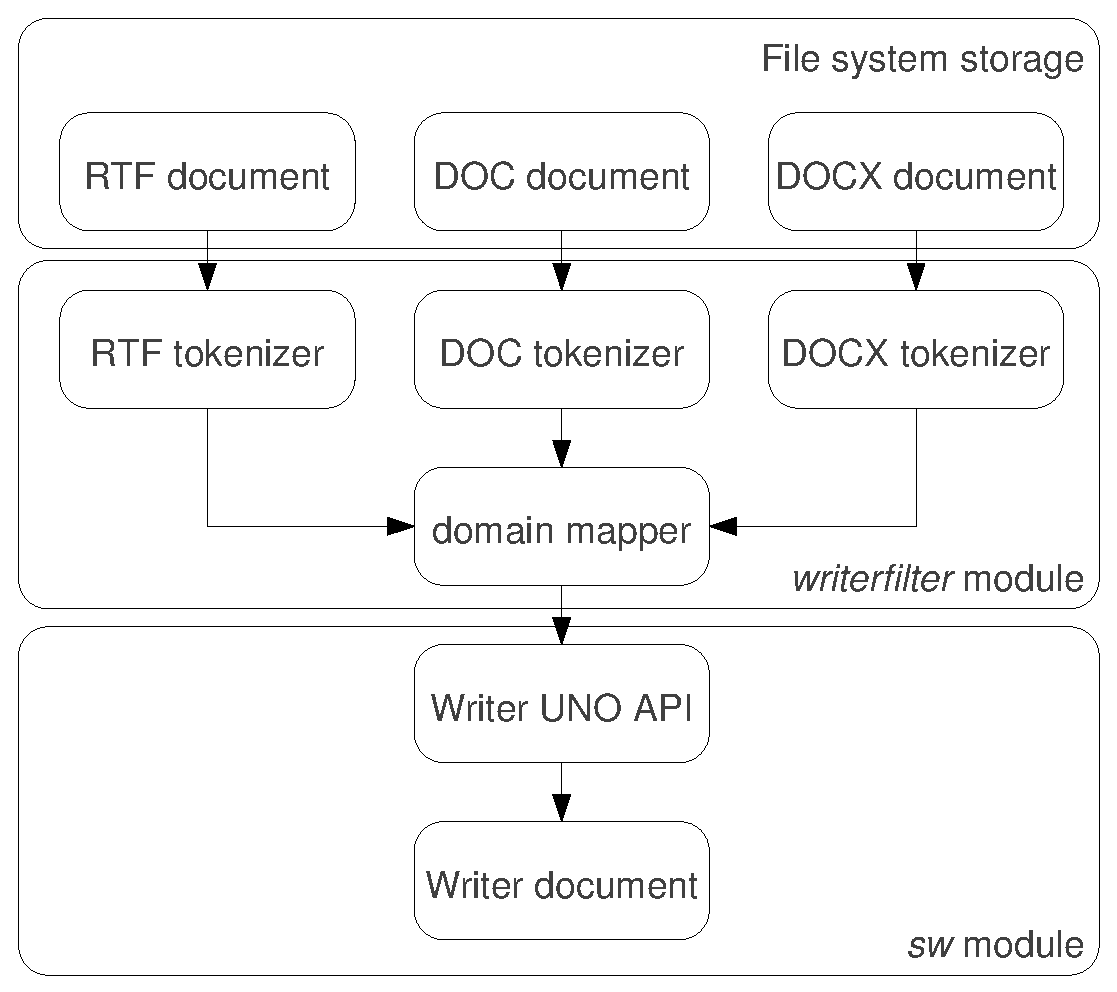
\includegraphics[width=50mm,keepaspectratio]{overview-architecture.eps}
\caption{Architecture of the RTF import filter}
\end{figure}

As it can be seen, my task had two major parts:

\begin{itemize}
\item Implementing an RTF tokenizer.
\item Improving the domain mapper as necessary.
\end{itemize}

The domain mapper provides the following interfaces, which has to be
implemented by a tokenizer:

\begin{itemize}
\item writerfilter::Reference<Stream> -- represents a file stream, that can be tokenized
\item writerfilter::Reference<Properties> -- represents a set of properties that modify the behaviour of text (font size)
\item writerfilter::Reference<Table> -- represents tables of settings at the start of document (list of fonts, styles, etc.)
\item Sprm -- represents a section, paragraph, or run (set of characters) modifier
\item Value -- represents a parameter of an Sprm
\end{itemize}

Once these interfaces are implemented, a filter implementation has to:

\begin{itemize}
\item Create a domain mapper instance, and pass the Writer UNO API document model to it.
\item Create a tokenizer instance, and pass file stream and the domain mapper instance to it.
\item Call the tokenizer's resolve() method to alter the document model to represent the contents of the file stream.
\end{itemize}

The tokenizer then has the following tasks:

\begin{itemize}
\item Send initial tables to the domain mapper.
\item Start/end sections, paragraphs, runs.
\item Wrap the tokenized parameters to Value instances, tokens to Sprm instances.
\item Send properties (set of sprms) at the start of sections, paragraphs or runs.
\end{itemize}

As a result, I designed the following tasks inside the RTF tokenizer library:

\begin{itemize}
\item RTFEncoding -- Helper for RTF legacy charsets.
\item RTFSymbol -- Respresents an RTF Control Word.
\item RTFDocumentFactory -- Hides RTFDocumentImpl behind an RTFDocument interface.
\item RTFDocument (inherited from writerfilter::Reference<Stream>) -- Pure virtual class, the filter can access only this one.
\item RTFDocumentImpl -- The implementation of RTFDocument, invokes the domain mapper based tokens got from RTFTokenizer.
\item RTFReferenceProperties (inherited writerfilter::Reference<Properties>) -- Sends RTFSprm instances to the domain mapper.
\item RTFReferenceTable (inherited from writerfilter::Reference<Table>) -- Sends tables (e.g. font table) to the domain mapper.
\item RTFSdrImport -- Helper to import drawings, uses the (Star)Draw UNO API.
\item RTFSkipDestination -- Helper to skip entire destinations if the destination control word is unhandled.
\item RTFSprms -- Contains a set of RTFSprm, used by RTFReferenceProperties.
\item RTFSprm (inherited from Sprm) -- represents an RTF control word.
\item RTFTokenizer -- The core of the tokenizer, knows only how to separate control words (and their parameters) from text.
\item RTFValue (inherited from Value) -- represents a parameter to an RTF control word.
\end{itemize}

Note that a set of sprms can be a tree in fact, as a Value can point to a set
of sprms as well, recursively.

\section{Implementation}

\subsection*{General}

The majority of the work was about re-creating an RTF tokenizer that supports
the same set of features as the old filter, except with a cleaner design,
making it possible to get rid of ugly hacks. Two such example:

\begin{itemize}
\item RtfReader -- the old filter -- used to hardcode the type of the control
words, RTFTokenizer now has this in a central table (originally generated from
the specification), making it impossible to handle incorrectly the parameters
of control words (e.g. handle the parameter of a value as a toggle).
\item RTFTokenizer separates the task of separating control words and text, for
example the meaning of the special \textbraceleft character is defined at a
single place, while it was handled in 19 (!) different places in RtfReader.
\end{itemize}

\subsection*{Fixed bugs}

My RTF improvements can be separated to bugfixes and features.

I fixed bugs in the following topics:

\begin{itemize}
\item Comments are not displayed upon saving and reopening RTF, are lost on
re-saving \cite{fdo36877}
\item Group containing tabs deletes previous tabs \cite{fdo36922}
\item Changing imported RTF tilts orientation of text \cite{fdo35985}
\item Subscripts in RTF from LaTex file are missing \cite{fdo36089}
\item Embedded picture invisible, rendering messed up\cite{fdo37691}
\end{itemize}

\subsection*{New features}

Once I was ready with an RTF filter that was as good as the old one, I worked on the following new features:

\begin{itemize}
\item character properties: blinking, relative font size in superscript characters
\item tables: nested tables, vertical merged cells
\item footnotes/endnotes: all characters of the foot/endnote mark are in the field, the field is properly superscript
\item sections: line numbering
\item fields: postit comments
\item Drawing objects for Word 97 through Word 2007 (shapes) are now handled:
\begin{itemize}
\item basic shapes (rectangle, ellipse, etc.)
\item lines, including free-form ones
\item texts, including vertical ones and their (paragraph and character) formatting
\end{itemize}
\item form fields: all types supported by the RTF format are handled
\item OLE objects: Their result is imported as a picture - RtfReader did not
import anything. When native is available, then it's handled as well, but no
automatic conversion is done yet (for DOC files there is an automatic
conversion from MathType to Writer formula).
\item text frames:
\begin{itemize}
\item anchor type is now parsed by RTFTokenizer (no longer always assume
\emph{to paragraph} but also handle \emph{as character})
\item handling of invalid nested frames now match the behaviour of Word
\end{itemize}
\end{itemize}

\subsection*{DOCX changes}

Given that the domain mapper operates on tokens and the tokens are derived from
the DOCX specification, the domain mapper is highly DOCX-specific. That means
that when the developer documentation is lacking, usually the best is to see
how the domain mapper works with DOCX documents, then other tokenizers can do
the same. As a result, I also fixed bugs in the domain mapper, improving DOCX
support in general. Here are a few items I added support for:

\begin{itemize}
\item double strikethrough character property used to have an effect till the
end of document (!)
\item text-to-text alignment is now imported
\item restart of footnote numbers
\item extra paragraph at the end of footnotes is no longer inserted
\end{itemize}

\section{Testing}

LibreOffice supports two kind of automated test types:

\begin{itemize}
\item unit tests
\item subsequent tests
\end{itemize}

Unit tests are always executed at the end of the build of a module, the failure
of them is considered a kind of build failure. This makes them quite useful,
however their scope is a bit limited: they can't use UNO services from module
they don't build-depend on.

Subsequent tests are however executed manually, once the complete product is
built. Given that most developers don't run these tests (as they are not forced
to), it's less useful, but these tests can use all UNO services.

In case of RTF import, I decided to implement unit tests. I make the domain
mapper handle the lack of Writer services handle gently (i.e. notice the lack
of existence, but don't fail) and this way a unit test could make sure the
import of an RTF document results in the expected return code, but it says
little about the actual rendered layout.

LibreOffice uses the CppUnit framework for unit testing. Given that I wanted to
be sure adding new test documents do not require code modifications, I defined
the following document classes:

\begin{itemize}
\item pass: the document should be imported without any error
\item fail: the import should return a proper error code (should not crash)
\item indeterminate: the importer should just not crash
\end{itemize}

The idea is that directories can represent the given document classes, and each
document in that directory is checked if the desired behaviour is achieved.

Creating test documents was the next step. During development, I followed a
test-driven approach, so I already had documents which should be imported
without errors in the following categories:

\begin{itemize}
\item hello world
\item character properties
\item character styles
\item paragraph properties
\item unicode support
\item numberings
\item pictures
\item tables
\item sections
\item headers and footers
\item footnotes
\item line numbering
\item bookmarks
\item tabla of contents
\item red lines (change tracking)
\item fields
\item drawing objects
\item forms
\item OLE objects: replacement graphics
\item OLE objects: load native data
\end{itemize}

For failing samples, I looked up what security advisories of
the product referred to the RTF importer earlier: that provided test documents
which should fail with a proper error.

Last, I needed a huge collection of RTF sample documents which I could throw in
the indeterminate directory: for that I used an existing Python script that
collected doc files from public bugzilla entries. With little modification I
modified it to use crawl rtf samples.

\section{Future work}

At the end of the internship I did some measurements about how many percent of
the control words are implemented from the specification. Of course that number
does not mention how relevant a keyword is: e.g. a drawing keyword not used
since Word 6.0 is way less important than a character property that sets the
current run as bold.

Version 1.9.1 of the specification contains 1815 control words, while the RTF
import filter at the time of writing parses 385 of them. That alone means that
there are plenty of possibilities to improve the filter.

However, there are smaller tasks which could be implemented, once the domain
mapper would support them:

\begin{itemize}
\item protected sections
\item page breaks: even/odd ones
\item make DomainMapper\_Impl :: PushPageHeader() handle ``left'' and ``all'' headers separately for RTF
\item NS\_ooxml :: LN\_EG\_SectPrContents\_pgNumType is completely ignored (page numbering style, restart)
\item OLE objects: convert native data (mathtype to mathml, etc), like the doc import does
\item crop of images is ignored
\end{itemize}

Additionally a performance idea: currently each control word is converted to a
numeric constant, which is then parsed by based on the type of the control
word. Converting to a constant means reading lines of a static array, comparing
the string value of the control word and the current entry, and then reading
the numeric value, if they match. This can be quite slow for large documents,
using gperf instead would be a better solution.\footnote{It's a code generator
that generates perfect hashes: so looking up the numeric constant in a table
based on string value would cost a single string comparison only.}

\clearpage

\begin{thebibliography}{4}
\addcontentsline{toc}{section}{References}

\bibitem{libreoffice} Libreoffice, http://libreoffice.org/
\bibitem{rtf} Word 2007: Rich Text Format (RTF) Specification, version 1.9.1, http://bit.ly/qD1CTV
\bibitem{fdo36877} https://bugs.freedesktop.org/show\_bug.cgi?id=36877
\bibitem{fdo36922} https://bugs.freedesktop.org/show\_bug.cgi?id=36922
\bibitem{fdo35985} https://bugs.freedesktop.org/show\_bug.cgi?id=35985
\bibitem{fdo36089} https://bugs.freedesktop.org/show\_bug.cgi?id=36089
\bibitem{fdo37691} https://bugs.freedesktop.org/show\_bug.cgi?id=37691

\end{thebibliography}

\end{document}
